\chapter{Wizja aplikacji}

\section{Wymagania funkcjonalne}
Tworzenie aplikacji należało zacząć od nakreślenia zakresu funkcjonalności, które aplikacja będzie udostępniać użytkownikom. Podstawowym zadaniem, które musi spełniać jest możliwość przeprowadzania eksperymentów przy pomocy systemu GDT. Kolejnym ważnym aspektem jest możliwość zarządzania, wyświetlania, udostępniania oraz edycji poszczególnych eksperymentów. Każdy z użytkowników powinien konkretnie widzieć, które z przeprowadzanych przez niego doświadczeń zostały już ukończone, a które jeszcze są w trakcie lub czekają w kolejce do obliczeń. Aplikacja powinna również przede wszystkim w przejrzysty sposób wyświetlać wyniki doświadczenia w postaci wygenerowanego drzewa decyzyjnego i poszczególnych statystyk. Podczas uruchomienia nowego zadania do obliczenia, użytkownikowi zostanie wyświetlony pasek postępu oraz oszacowana długość trwania całego zadania, przy czym w dowolnym momencie będzie mógł anulować polecenie.  Wraz z możliwością tworzenia eksperymentu nie odłącznym elementem będzie funkcjonalność zarządzania plikami wejściowymi oraz wyjściowymi. Dla użytkowników początkujących zostanie przedstawiona opcja tworzenia podstawowych plików konfiguracyjnych, bez wgłębiania się w bardziej zaawansowane parametry eksperymentu. Dostęp do całości funkcjonalności powinien być tylko dostępny dla zarejestrowanych użytkowników. Natomiast możliwość rejestracji oraz logowania będzie ogólnodostępna.

System kont użytkowników powinien wyróżniać różne role, które definiowałyby dostęp do poszczególnych funkcjonalności aplikacji. Zarządzanie tymi uprawnieniami będzie się odbywać po przez panel administratora. Administrator aplikacji dodatkowo może modyfikować oraz usuwać konta użytkowników. Co więcej z interfejsu admina będzie istniała możliwość edycji rekordów z bazy danych oraz edycja uprawnień do poszczególnych eksperymentów. 

Biorą pod uwagę możliwość udostępniania przez użytkownika doświadczenia innemu użytkownikowi, ważnym aspektem będzie umożliwienie ograniczenia części akcji możliwych do wykonania na eksperymencie. Podstawowym uprawnieniem, którego nie da się zablokować będzie możliwość wyświetlenia wyników eksperymentu. Natomiast reszta funkcjonalności możliwych do wykonania na doświadczeniu, takich jak uruchamianie, kopiowanie, edycja, usuwanie czy też pobieranie plików wejściowych lub wyjściowych może zostać ograniczona. Użytkownik posiadający od kogoś udostępniony eksperyment z pewnymi ograniczeniami, może udostępnić go dalej tylko jeśli posiada nadane prawa do udostępniania, przy czym nie może znieść już nadanych wcześniej ograniczeń.


\begin{figure}[htb]
\centering
\includegraphics[width=11cm]{grafika/diagram_przypadkow_uzycia.eps}
\caption{Diagram przypadków użycia, źródło: opracowanie własne}
\label{rys1_diagram_przypadkow}
\end{figure}

\begin{figure}[htb]
	\centering
	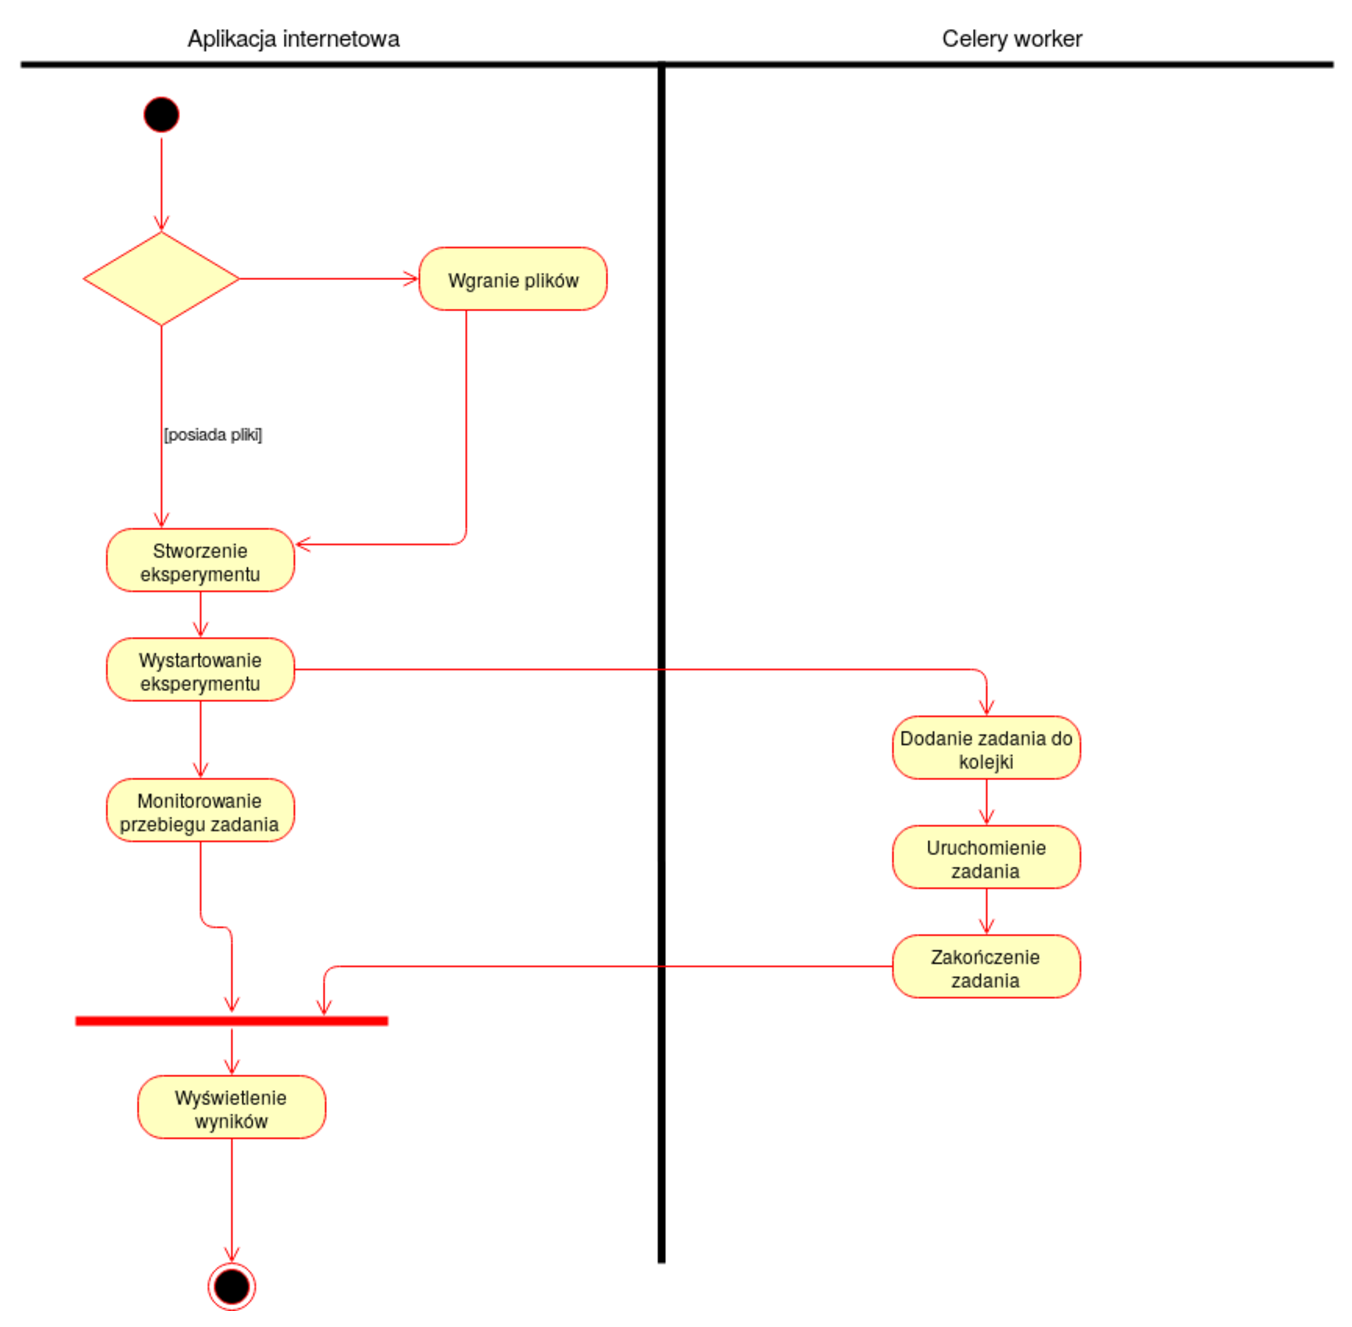
\includegraphics[width=11cm]{grafika/diagram_przebiegu_tworzenia_eksperymentu.eps}
	\caption{Diagram czynności tworzenia i uruchomiania eksperymentu, źródło: opracowanie własne}
	\label{rys2_diagram_czynności}
\end{figure}

Na rysunku \ref{rys1_diagram_przypadkow} przedstawiono wszystkie funkcjonalności w postaci diagramu przypadków użycia. W aplikacji zostały wyszczególnione trzy role dostępne do uzyskania dla każdego użytkownika oraz rola administratora całego systemu. Wszystkie przypadki użycia oprócz logowania i rejestracji są dostępne tylko dla użytkowników zalogowanych. Każdy nowy użytkownik musi założyć konto, aby mieć dostęp do aplikacji. Nowo powstałe konta otrzymują uprawnienia na domyślnym poziomie "1\_default", a wyższe poziomy uprawnień mogą zostać nadane po przez administratora. Kolejne role rozszerzają możliwości użytkownika pod względem ilości akcji możliwych do wykonania. Poziom "2\_exp"\ umożliwia tworzenie nowych eksperymentów, przy czym tylko najwyższy poziom uprawnień "3\_exp\_data"\  pozwala na wgrywanie plików do aplikacji. Przebieg czynności związanych ze stworzeniem nowego eksperymentu oraz wyświetleniem wyników został przedstawiony na rysunku \ref{rys2_diagram_czynności}. 



Opis przypadku użycia "Tworzenie nowego eksperymentu":
\begin{enumerate}
\item  Aktor
	\begin{itemize}
		\item Użytkownik. 
	\end{itemize}
\item Warunki początkowe
	\begin{itemize}
		\item Aktor jest zalogowany oraz posiada uprawnienia przynajmniej na poziomie "2\_exp".
	\end{itemize}
\item Zdarzenie inicjujące
	\begin{itemize}
		\item Naciśnięcie przycisku "New experiment" nad listą wszystkich eksperymentów użytkownika.
	\end{itemize}
\item Przebieg w krokach
	\begin{itemize}
		\item Aplikacja przechodzi do formularza tworzenia nowego eksperymentu,
		\item Użytkownik wypełnia i zatwierdza formularz.
	\end{itemize}
\item Przebiegi alternatywne
	\begin{itemize}
		\item  Użytkownik nie uzupełnia wszystkich pól formularza, aplikacja wyświetla powiadomienie o pustych polach.
	\end{itemize}
\item Sytuacje wyjątkowe
	\begin{itemize}
		\item  Użytkownik nie posiada żadnych plików wgranych do aplikacji. Powoduje to, że pola formularza zawierające pliki są puste. Uniemożliwia to stworzenie nowego eksperymentu, a aplikacja wyświetla powiadomienie o pustych polach przy podjętej próbie zatwierdzenia.
	\end{itemize}
\item Warunki końcowe
	\begin{itemize}
		\item  System przekierowuje użytkownika do listy z eksperymentami, a na liście znajduje się nowo utworzony eksperyment.
	\end{itemize}
\item Zależności czasowe
	\begin{itemize}
		\item  Częstotliwość wykonywania: Około 20 razy dziennie na każdego użytkownika,
		\item Typowy czas realizacji: 8 sekund.
	\end{itemize}
\end{enumerate}

Opis przypadku użycia "Wystartowanie eksperymentu":
\begin{enumerate}
	\item  Aktor
	\begin{itemize}
		\item Użytkownik. 
	\end{itemize}
	\item Warunki początkowe
	\begin{itemize}
		\item Aktor jest zalogowany oraz posiada stworzony eksperyment.
	\end{itemize}
	\item Zdarzenie inicjujące
	\begin{itemize}
		\item Naciśnięcie przycisku "Show" w liście eksperymentów na elemencie, którego status to "Created".
	\end{itemize}
	\item Przebieg w krokach
	\begin{itemize}
		\item Aplikacja przechodzi do podglądu szczegółów wybranego eksperymentu,
		\item Użytkownik klika przycisk "Start" znajdujący się na pasku możliwych czynności,
		\item Aplikacja przekierowuje użytkownika do listy eksperymentów.
	\end{itemize}
	\item Przebiegi alternatywne
	\begin{itemize}
		\item  Po wystartowaniu eksperymentu nastąpił błąd i jest to sygnalizowane zmianą statusu na "Error", a w szczegółach eksperymentu można podejrzeć wiadomość z błędem.
	\end{itemize}
	\item Sytuacje wyjątkowe
	\begin{itemize}
		\item  Użytkownikowi nie posiada prawd do wystartowania konkretnego eksperymentu i w panelu akcji nie wyświetla się przycisk Start".
	\end{itemize}
	\item Warunki końcowe
	\begin{itemize}
		\item  Eksperyment zmienił swój status na "In queue"\ lub "Running", a po przejściu do szczegółów wyświetla się pasek postępu oraz szacowany czas oczekiwania na zakończenie.
	\end{itemize}
	\item Zależności czasowe
	\begin{itemize}
		\item Częstotliwość wykonywania: Około 20 razy dziennie na każdego użytkownika,
		\item Typowy czas realizacji: 8 sekund.
	\end{itemize}
\end{enumerate}

Opis przypadku użycia "Wyświetlenie drzewa wynikowego":
\begin{enumerate}
	\item  Aktor
	\begin{itemize}
		\item Użytkownik. 
	\end{itemize}
	\item Warunki początkowe
	\begin{itemize}
		\item Aktor jest zalogowany oraz posiada ukończony eksperyment.
	\end{itemize}
	\item Zdarzenie inicjujące
	\begin{itemize}
		\item Naciśnięcie przycisku "Show" w liście eksperymentów na elemencie, którego status to "Finished".
	\end{itemize}
	\item Przebieg w krokach
	\begin{itemize}
		\item Aplikacja przechodzi do podglądu szczegółów wybranego eksperymentu, a na samym dole karty wyświetlają się linki do drzew decyzyjnych,
		\item Użytkownik klika w link do drzewa decyzyjnego.
	\end{itemize}
	\item Przebiegi alternatywne
	\begin{itemize}
		\item  Brak.
	\end{itemize}
	\item Sytuacje wyjątkowe
	\begin{itemize}
		\item  Brak.
	\end{itemize}
	\item Warunki końcowe
	\begin{itemize}
	\item  Aplikacja wyświetliła drzewo decyzyjne wraz ze statystykami.
	\end{itemize}
	\item Zależności czasowe
	\begin{itemize}
		\item Częstotliwość wykonywania: Około 30 razy dziennie na każdego użytkownika,
		\item Typowy czas realizacji: 10 sekund.
	\end{itemize}
\end{enumerate}

\section{Wymagania niefunkcjonalne}
asdasd.
\section{Wykorzystane technologie}
asdasd.